%% LyX 2.3.6.1 created this file.  For more info, see http://www.lyx.org/.
%% Do not edit unless you really know what you are doing.
\documentclass[12pt,english,brazil]{article}
\usepackage[T1]{fontenc}
\usepackage[latin9]{inputenc}
\usepackage[a4paper]{geometry}
\geometry{verbose,tmargin=1.5cm,bmargin=2cm,lmargin=2cm,rmargin=2cm,headheight=0cm,headsep=0cm}
\setcounter{secnumdepth}{4}
\setlength{\parskip}{\medskipamount}
\setlength{\parindent}{0pt}
\usepackage{xcolor}
\usepackage{array}
\usepackage{verbatim}
\usepackage{float}
\usepackage{fancybox}
\usepackage{calc}
\usepackage{textcomp}
\usepackage{graphicx}
\PassOptionsToPackage{normalem}{ulem}
\usepackage{ulem}

\makeatletter

%%%%%%%%%%%%%%%%%%%%%%%%%%%%%% LyX specific LaTeX commands.
%% Because html converters don't know tabularnewline
\providecommand{\tabularnewline}{\\}

\@ifundefined{date}{}{\date{}}
%%%%%%%%%%%%%%%%%%%%%%%%%%%%%% User specified LaTeX commands.
% Carga do pacote SisDig.
%	Alterações de formatações deverão ser realizadas,
%   preferencialmente, no pacote -- a não ser que seja
%   algo muito específico para provas.
\usepackage{../3.1-bibliotecas/latex/sisdig}

\makeatother

\usepackage{babel}
\begin{document}
\begin{comment}
Macros
\end{comment}

\global\long\def\six#1#2{\SI{#1}{#2}}%

\newcommand{\caixaresp}[1][10]{%

\medskip{}

\begin{tabular}{|>{\centering}p{1\linewidth}|}
\hline 
\espv[#1]\tabularnewline
\hline 
\end{tabular}

}

\begin{comment}
\textbf{=== Capa de Prova (dg) ===}
\end{comment}

%Capa
% Parâmetros: prova, ano, data, qtd. questões.
\newcommand{\capadg}[4]{%
\begin{center}
\begin{center}
\textsc{\LARGE{}
\includegraphics[height=1.4cm]{imagens/logo-imt}\quad{}}%
\begin{minipage}[b][1\totalheight][c]{12cm}%
\textsc{\Large{}ETE102\smallskip{}
}\\
\textsc{\Large{}Fundamentos de Circuitos Digitais}%
\end{minipage}\textsc{\LARGE{}\vspace{1.5cm}
}\\
\textsc{\LARGE{}#1 de #2}{\LARGE\par}
\par\end{center}

\begin{center}
\textsc{\LARGE{}Período Noturno}{\LARGE\par}
\par\end{center}

\begin{center}
{\large{}\vspace{3.5ex}
Profº Marcelo Porto Trevizan\bigskip{}
}\marginpar{10,0

\bigskip{}

9,5

\bigskip{}

9,0

\bigskip{}

8,5

\bigskip{}

8,0\bigskip{}

7,5\bigskip{}

7,0

\bigskip{}

6,5

\bigskip{}

6,0

\bigskip{}

5,5

\bigskip{}

5,0

\bigskip{}

4,5

\bigskip{}

4,0\bigskip{}

3,5\bigskip{}

3,0

\bigskip{}

2,5

\bigskip{}

2,0

\bigskip{}

1,5

\bigskip{}

1,0

\bigskip{}

0,5

\bigskip{}

0,0}
\par\end{center}

\begin{tabular}{rlrc}
Nome: & \uline{\hspace{8cm}} & RA: & \uline{\hspace{3cm}}\tabularnewline
 &  &  & \tabularnewline
Assinatura: & \uline{\hspace{8cm}} & Data: & #3\tabularnewline
\end{tabular}

\bigskip{}


\section*{Orientações:}
\begin{itemize}
\item Prova sem consulta; 
\item não é permitido o uso de calculadoras;
\item respostas a lápis ou caneta;
\item as questões que o possuírem, deverão ter sua resposta final no espaço
reservado;
\item contém #4 questões;
\item duração de 90 min.;
\item por gentileza, \emph{desligar os celulares};
\item pontuação máxima de 10,0 pontos.
\end{itemize}
\vfill{}

\begin{center}
\texttt{\emph{\Huge{}Boa Prova!!!}}{\Huge\par}
\par\end{center}

\begin{center}
\vfill{}
\thispagestyle{empty}\newpage{}
\par\end{center}

\emph{(Espaço reservado para rascunho. Poderá ser utilizado para continuar
questão, desde que }\emph{\uline{devidamente}}\emph{ identificada.)}

\phantom{}

\newpage{}
\par\end{center}

} %\capa

\begin{comment}
\textbf{=== Capa de Prova (an) ===}
\end{comment}

%Capa
% Parâmetros: prova, ano, data, qtd. questões.
\newcommand{\capaan}[4]{%
\begin{center}
\begin{center}
\textsc{\LARGE{}
\includegraphics[height=1.4cm]{imagens/logo-imt}\quad{}}%
\begin{minipage}[b][1\totalheight][c]{12cm}%
\textsc{\Large{}ETE103\smallskip{}
}\\
\textsc{\Large{}Fundamentos de Circuitos Analógicos}%
\end{minipage}\textsc{\LARGE{}\vspace{1.5cm}
}\\
\textsc{\LARGE{}#1 de #2}{\LARGE\par}
\par\end{center}

\begin{center}
\textsc{\LARGE{}Período Noturno}{\LARGE\par}
\par\end{center}

\begin{center}
{\large{}\vspace{3.5ex}
Profº Marcelo Porto Trevizan\bigskip{}
}\marginpar{\protect\begin{center}
\textcolor{lightgray}{\pontuacoes[-50]{10}{00}}\protect
\par\end{center}}
\par\end{center}

\begin{tabular}{rlrc}
Nome: & \uline{\hspace{8cm}} & RA: & \uline{\hspace{3cm}}\tabularnewline
 &  &  & \tabularnewline
Assinatura: & \uline{\hspace{8cm}} & Data: & #3\tabularnewline
\end{tabular}

\bigskip{}

\begin{center}
\textbf{\Large{}Orientações}{\Large\par}
\par\end{center}
\begin{itemize}
\item Prova sem consulta; 
\item é permitido o uso de qualquer calculadora;
\item respostas a lápis ou caneta;
\item as questões que o possuírem, deverão ter sua resposta final no espaço
reservado;
\item todas as questões devem possuir a correspondente justificativa e/ou
o os cálculos, conforme o contexto;
\item contém #4 questões;
\item duração de 90 min.;
\item por gentileza, \emph{desligar os celulares};
\item pontuação máxima de 10,0 pontos.
\end{itemize}
\vfill{}

\begin{center}
\texttt{\emph{\Huge{}Boa Prova!!!}}{\Huge\par}
\par\end{center}

\begin{center}
\vfill{}
\thispagestyle{empty}\newpage{}
\par\end{center}

\emph{(Espaço reservado para rascunho. Poderá ser utilizado para continuar
questão, desde que }\emph{\uline{devidamente}}\emph{ identificada.)}

\phantom{}

\newpage{}
\par\end{center}

} %\capa

\begin{comment}
\textbf{=== Capa de Trabalho Substituto de Prova (an) ===}
\end{comment}

%Capas de trabalho substituto de prova
% Parâmetros: prova, ano, data, qtd. questões.
\newcommand{\capaant}[4]{%
\begin{center}
\begin{center}
\textsc{\LARGE{}
\includegraphics[height=1.4cm]{imagens/logo-imt}\quad{}}%
\begin{minipage}[b][1\totalheight][c]{12cm}%
\textsc{\Large{}ETE103\smallskip{}
}\\
\textsc{\Large{}Fundamentos de Circuitos Analógicos}%
\end{minipage}\textsc{\LARGE{}\vspace{1.5cm}
}\\
\textsc{\LARGE{}#1 de #2}{\LARGE\par}
\par\end{center}

\begin{center}
\textsc{\LARGE{}Período Noturno}{\LARGE\par}
\par\end{center}

\begin{center}
{\large{}\vspace{3.5ex}
Profº Marcelo Porto Trevizan\bigskip{}
}\marginpar{\protect\begin{center}
\textcolor{lightgray}{\pontuacoes[-50]{10}{00}}\protect
\par\end{center}}
\par\end{center}

\begin{tabular}{rlrc}
Nome: & \uline{\hspace{8cm}} & RA: & \uline{\hspace{3cm}}\tabularnewline
 &  &  & \tabularnewline
Assinatura: & \uline{\hspace{8cm}} & Data: & #3\tabularnewline
\end{tabular}

\bigskip{}

\begin{center}
\textbf{\Large{}Orientações}{\Large\par}
\par\end{center}
\begin{itemize}
\item Este trabalho substituto de prova é \textbf{individual};
\item por favor, resolver de forma organizada e destacar as respostas;
\item as questões possuem valores parametrizados por RA, conforme tabelas
no arquivo \texttt{}~\linebreak{}
\texttt{ete103-n-p1-2020-valores-por-ra.ods}, disponível no Moodle;
\textbf{muita atenção!}, pois o uso de valor incorreto implicará em
desconto de 50\% na nota da questão;
\item por favor, indicar, com destaque, o valor dos parâmetros utilizados
obtidos da tabela;
\item contém #4 questões;
\item o prazo para entrega é até as 23h59 da data final apontada no cabeçalho
acima;
\item o arquivo de entrega deverá estar em formato PDF;
\item o enunciado deverá fazer parte do arquivo enviado; folhas avulsas
poderão ser intercaladas entre uma questão e outra;
\item pontuação máxima de 10,0 pontos.
\end{itemize}
\vfill{}

\begin{center}
\texttt{\emph{\Huge{}Bom Trabalho!!!}}{\Huge\par}
\par\end{center}

\begin{center}
\vfill{}
\thispagestyle{empty}\newpage{}
\par\end{center}

\emph{(Espaço reservado para rascunho. Poderá ser utilizado para continuar
questão, desde que }\emph{\uline{devidamente}}\emph{ identificada.)}

\phantom{}

\newpage{}
\par\end{center}

} %\capaant

\begin{comment}
\textbf{=== Capas Genéricas de Trabalho e Prova com Acordo ===}
\end{comment}

\newcommand{\capaacordo}[6]{\begin{center}
\textsc{\LARGE{}
\includegraphics[height=1.4cm]{imagens/logo-imt}\quad{}}%
\begin{minipage}[b][1\totalheight][c]{12cm}%
\textsc{\Large{}#5\smallskip{}
}\\
\textsc{\Large{}#6}%
\end{minipage}\textsc{\LARGE{}\vspace{1.5cm}
}\\
\textsc{\LARGE{}#1 de #2}{\LARGE\par}
\par\end{center}

\begin{center}
\textsc{\LARGE{}Período Noturno}{\LARGE\par}
\par\end{center}

\begin{center}
{\large{}\vspace{3.5ex}
Profº Marcelo Porto Trevizan\bigskip{}
}\marginpar{\protect\begin{center}
\textcolor{lightgray}{\pontuacoes[-50]{10}{00}}\protect
\par\end{center}}
\par\end{center}

\begin{tabular}{rlrc}
Nome: & \uline{\hspace{8cm}} & RA: & \uline{\hspace{3cm}}\tabularnewline
 &  &  & \tabularnewline
Assinatura: & \uline{\hspace{8cm}} & Data: & #3\tabularnewline
\end{tabular}

\bigskip{}

\begin{center}
\textbf{\Large{}Orientações}{\Large\par}
\par\end{center}
\begin{itemize}
\item Este trabalho é \textbf{individual};
\item \textcolor{blue}{este trabalho será válido apenas se o cabeçalho acima
e o }\textbf{\textcolor{blue}{Acordo de Ética }}\textcolor{blue}{abaixo
estiverem assinados;}
\item a tentativa identificada de plágio ou fraude poderá acarretar em nota
zero na questão ou na prova inteira;
\item por favor, resolver de forma organizada e destacar as respostas;
\item contém #4 questão;
\item não é obrigatória a resolução de todas as questões;
\item o prazo para entrega é até as 23h59 da data final apontada no cabeçalho
acima;
\item o arquivo de entrega deverá estar em formato PDF;
\item \uline{o enunciado deverá fazer parte do arquivo enviado}; folhas
avulsas poderão ser intercaladas entre uma questão e outra;
\item apresentar as resoluções de forma manuscrita;
\item \textbf{todas as resoluções devem ser acompanhadas de cálculos e justificativas,
conforme o que for pertinente, salvo sob outra orientação no enunciado
da própria questão;}
\item pontuação máxima de 10,0 pontos, com direito a duas entregas, conforme
explanado em aula.
\end{itemize}
\begin{center}
\thispagestyle{empty}
\par\end{center}
\begin{quote}
\begin{flushleft}
\textbf{\large{}\newpage}%
{\fboxsep 2ex\ovalbox{\begin{minipage}[t]{0.83\columnwidth}%
\begin{quote}
\begin{center}
\textbf{\large{}Acordo de Ética}{\large\par}
\par\end{center}
\texttt{\emph{A ética nasce no berço, caminha pela escola e acompanha
toda a vida pessoal e profissional de cada pessoa.}}

Ciente da questão ética que nos permeia e de que \uline{este trabalho
substituto de prova é individual}, declaro que não cometerei qualquer
tipo fraude ou plágio em sua resolução.\bigskip{}
\end{quote}
\begin{center}
\begin{tabular}{c}
\uline{\hspace{8cm}}\tabularnewline
Assinatura\tabularnewline
\end{tabular}
\par\end{center}%
\end{minipage}}}
\par\end{flushleft}
\textbf{Nota sobre o Acordo de Ética}

É possível interagir com um colega a respeito do conteúdo do trabalho
e este \textbf{pode dar uma dica} para sua resolução. Todavia \textbf{não
poderá fornecer a resolução das questões, total ou parcial}, seja
por qual forma for.

Por exemplo, o colega poderá dizer ``use o conceito Z'', ou ``consulte
o capítulo N do livro X'', mas não poderá ditar ou fornecer uma cópia
da expressão que ele usou para resolver o exercício, nem a resposta
final.
\end{quote}
\vfill{}

\begin{center}
\scalebox{2}[2]{\texttt{\emph{\Huge{}Bom Trabalho!!!}}}
\par\end{center}

\begin{center}
\vfill{}
\thispagestyle{empty}\newpage{}
\par\end{center}} %\capaacordo

\newcommand{\capaacordoprova}[6]{\begin{center}
\textsc{\LARGE{}
\includegraphics[height=1.4cm]{imagens/logo-imt}\quad{}}%
\begin{minipage}[b][1\totalheight][c]{12cm}%
\begin{flushleft}
\textsc{\Large{}#5\smallskip{}
}\\
\textsc{\Large{}#6}
\par\end{flushleft}%
\end{minipage}\textsc{\LARGE{}\vspace{1.5cm}
}\\
\textsc{\LARGE{}#1 de #2}{\LARGE\par}
\par\end{center}

\begin{center}
\textsc{\LARGE{}Período Noturno}{\LARGE\par}
\par\end{center}

\begin{center}
{\large{}\vspace{3.5ex}
Profº Marcelo Porto Trevizan\bigskip{}
}\marginpar{\protect\begin{center}
\textcolor{lightgray}{\pontuacoes[-50]{10}{00}}\protect
\par\end{center}}
\par\end{center}

\begin{tabular}{rlrc}
Nome: & \uline{\hspace{8cm}} & RA: & \uline{\hspace{3cm}}\tabularnewline
 &  &  & \tabularnewline
Assinatura: & \uline{\hspace{8cm}} & Data: & #3\tabularnewline
\end{tabular}

\bigskip{}

\begin{center}
\textbf{\Large{}Orientações}{\Large\par}
\par\end{center}
\begin{itemize}
\item Esta prova é \textbf{individual};
\item \textcolor{blue}{esta prova será válida apenas se o cabeçalho acima
e o }\textbf{\textcolor{blue}{Acordo de Ética }}\textcolor{blue}{abaixo
estiverem assinados;}
\item a tentativa identificada de plágio ou fraude poderá acarretar em nota
zero na questão ou na prova inteira;
\item por favor, resolver de forma organizada e destacar as respostas;
\item contém #4 questões;
\item não é obrigatória a resolução de todas as questões;
\item o prazo para entrega é até 30 minutos após o horário final apontado
no cabeçalho acima;
\item o arquivo de entrega deverá estar em formato PDF;
\item \uline{o enunciado deverá fazer parte do arquivo enviado}; folhas
avulsas poderão ser intercaladas entre uma questão e outra;
\item apresentar as resoluções de forma manuscrita;
\item \textbf{todas as resoluções devem ser acompanhadas de cálculos e justificativas,
conforme o que for pertinente, salvo sob outra orientação no enunciado
da própria questão;}
\item a prova é com consulta;
\item pontuação máxima de 10,0 pontos.
\end{itemize}
\begin{center}
\thispagestyle{empty}
\par\end{center}
\begin{quote}
\begin{flushleft}
\textbf{\large{}\newpage}%
{\fboxsep 2ex\ovalbox{\begin{minipage}[t]{0.83\columnwidth}%
\begin{quote}
\begin{center}
\textbf{\large{}Acordo de Ética}{\large\par}
\par\end{center}
\texttt{\emph{A ética nasce no berço, caminha pela escola e acompanha
toda a vida pessoal e profissional de cada pessoa.}}

Ciente da questão ética que nos permeia e de que \uline{esta prova
é individual}, declaro que não cometerei qualquer tipo fraude ou plágio
em sua resolução.\bigskip{}
\end{quote}
\begin{center}
\begin{tabular}{c}
\uline{\hspace{8cm}}\tabularnewline
Assinatura\tabularnewline
\end{tabular}
\par\end{center}%
\end{minipage}}}
\par\end{flushleft}
\textbf{\phantom{}}

\textbf{\bigskip{}
Nota sobre o Acordo de Ética para esta prova}

\hspace{0.5em}Não é permitida \textbf{NENHUMA INTERAÇÃO ENTRE OS
COLEGAS}.
\end{quote}
\vfill{}

\begin{center}
\scalebox{2}[2]{\textcolor{teal}{\texttt{\emph{\Huge{}Boa Prova!!!}}}}
\par\end{center}

\begin{center}
\vfill{}
\thispagestyle{empty}\newpage{}
\par\end{center}} %\capaacordo

\begin{comment}
\textbf{=== Capa de Trabalho com Acordo (dg) ===}
\end{comment}

\newcommand{\capadgtacordo}[4]{%
	\capaacordo{#1}{#2}{#3}{#4}{ETE102}{Fundamentos de Circuitos Digitais}
} % \capadgtacordo

\begin{comment}
\textbf{=== Capa de Prova com Acordo (dg) ===}
\end{comment}

\newcommand{\capadgpacordo}[4]{%
	\capaacordoprova{#1}{#2}{#3}{#4}{ETE102}{Fundamentos de Circuitos Digitais}
} % \capadgpacordo

\begin{comment}
\textbf{=== Capa com Acordo (an) ===}
\end{comment}

\newcommand{\capaantacordo}[4]{%
	\capaacordo{#1}{#2}{#3}{#4}{ETE103}{Fundamentos de Circuitos Analógicos}
} % \capaantacordo

\begin{comment}
\textbf{=== 2015 ===}
\end{comment}

\begin{comment}
dg
\end{comment}

\begin{comment}
an
\end{comment}

\begin{comment}
\textbf{=== 2016 ===}
\end{comment}

\begin{comment}
dg
\end{comment}

\begin{comment}
an
\end{comment}

\begin{comment}
\textbf{=== 2017 ===}
\end{comment}

\begin{comment}
dg
\end{comment}

\begin{comment}
an
\end{comment}

\begin{comment}
\textbf{=== 2018 ===}
\end{comment}

\begin{comment}
dg
\end{comment}

\begin{comment}
an
\end{comment}

\begin{comment}
\textbf{=== 2019 ===}
\end{comment}

\begin{comment}
dg
\end{comment}

\begin{comment}
an
\end{comment}

\begin{comment}
\textbf{=== 2020 ===}
\end{comment}

\begin{comment}
an
\end{comment}

\begin{comment}
\textbf{=== 2021 ===}
\end{comment}

\begin{comment}
dg
\end{comment}

\begin{comment}
an
\end{comment}

\begin{comment}
\textbf{=== 2022 ===}
\end{comment}

\begin{comment}
dg
\end{comment}

\begin{comment}
an
\end{comment}

\begin{comment}
\textbf{=== 2022 ===}
\end{comment}

\begin{comment}
dg
\end{comment}

\capadg{Prova Substitutiva}{2023}{01.08.2023 19h}{\ref{que:ultima-questao-dg-ps-2023}}


\section{\questao[3]{50} Quanto ao contador apresentado no circuito abaixo,
pede-se:}

{\alfaenum
\begin{enumerate}
\item \valor{0,25} Indicar o tipo de contador: assíncrono ou síncrono.\textcolor{red}{}\vspace{1cm}
\item \valor{1,5} Completar o circuito de tal forma que a contagem seja
crescente e cíclica de $(4)_{16}$ a $(E)_{16}$, incluindo o sinal
de POR.\begin{center}
\begin{figure}[H]
\centering{}%
\fbox{\begin{minipage}[t]{1\columnwidth - 2\fboxsep - 2\fboxrule}%
\begin{center}
\vspace{4cm}
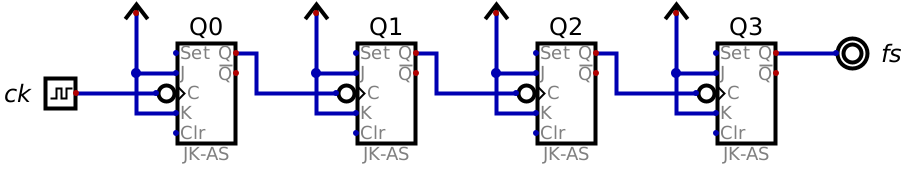
\includegraphics[width=0.8\textwidth]{imagens/2022/dg/p2/contador-assincrono-incompleto}\vspace{4cm}
\par\end{center}%
\end{minipage}}
\end{figure}
\par\end{center}
\item \valor{0,5} Traçar o Diagrama de Estados conforme percepção para
operar como um ``relógio de segundos''.\vspace{4cm}
\item \valor{0,5} Considerando-se $f_{s}$ como o sinal de saída, por quanto
a frequência do \foreignlanguage{english}{\emph{clock}} é dividida?
Apresente uma breve justificativa.\vspace{3cm}
\item \valor{0,75} Dado o trecho da carta de tempos abaixo, \textbf{sem
considerar os atrasos de propagação}, completá-la (\emph{considerar
o estado inicial indicado na carta: $(\mathrm{4})_{16}$}).
\end{enumerate}
\begin{center}
\begin{center}
\scalebox{2.0}[2.0]{%
\begin{tikztimingtable}[%
		timing/draw grid,
		timing/rowdist=2,
		timing/coldist=0.25,
		timing/name/.style={font=\normalfont\sffamily\scriptsize},
		timing/font=\bfseries\itshape,
		timing/wscale=2
	]
	$ck$		       		   & 12{C} \\
	$Q_0$						 & L; 11S \\
	$Q_1$						 & L; 11S \\
	$Q_2$						 & H; 11S \\
	$Q_3$						 & L; 11S \\	
\end{tikztimingtable}
}%
\bigskip
\par\end{center}
\par\end{center}

}

\section{\questao[1]{50} Dado o \foreignlanguage{english}{\emph{Latch}} \emph{Transparente}
de 2 bits apresentado, pede-se completar a Carta de Tempos.}
\begin{center}

\includegraphics[scale=0.5]{imagens/2023/p2/latch}\bigskip{}
\par\end{center}

\begin{center}
\begin{center}
\scalebox{2.5}[2.0]{%
\begin{tikztimingtable}[%
		timing/draw grid,
		timing/rowdist=2,
		timing/coldist=0.25,
		timing/name/.style={font=\normalfont\sffamily\scriptsize},
		timing/font=\bfseries\itshape,
		timing/wscale=0.5,
		timing/slope=0.0
	]
	$EN$		       		   & L	L	L	L	L	L	L	L	L	L	L	H	H	H	H	H	H	H	H	H	H	H	H	H	H	L	L	L	L	L	L	H	H	L	L\\
	$D_1$						 & L	H	L	H	L	L	L	H	H	L	L	L	H	L	L	L	L	L	L	H	H	H	H	L	H	H	L	H	L	H	L	L	L	L	L\\
	$D_0$						 & L	L	L	L	L	H	L	L	H	H	L	L	L	L	H	L	H	L	H	H	L	H	L	L	L	L	L	L	L	L	L	L	H	H	L\\
	$Q_1$						 & L; 34S \\
	$Q_0$						 & L; 34S \\	
\end{tikztimingtable}
}%
\bigskip
\par\end{center}
\par\end{center}

\section{\qquestao[2]{50} Deseja-se projetar um Contador Síncrono de 3 bits
utilizando \emph{flip-flops }JK. A sequência de contagem deste contador,
em binário, ciclicamente, é:\label{sec:dg-2023-p2Contador-Sincrono-JK-1}}
\begin{center}
010 \textemdash{} 001 \textemdash{} 011 \textemdash{} 100 \textemdash{}
111
\par\end{center}

Para tanto, pede-se:

\alfaenum{
\begin{enumerate}
\item \valor{0,5} Diagrama de Estados (\emph{indicar o estado inicial após
o POR!}).\vspace{5cm}
\item \valor{1,0} Tabela de Transição de Estados.\medskip{}
\\
\phantom{}\hfill{}{\esptab%
\begin{tabular}{>{\centering}m{0.6cm}>{\centering}m{0.6cm}>{\centering}m{0.6cm}|>{\centering}m{0.6cm}>{\centering}m{0.6cm}>{\centering}m{0.6cm}|>{\centering}m{0.6cm}>{\centering}m{0.6cm}|>{\centering}m{0.6cm}>{\centering}m{0.6cm}|>{\centering}m{0.6cm}>{\centering}m{0.6cm}}
\hline 
\multicolumn{3}{c|}{Est. Pres.} & \multicolumn{3}{c|}{Est. Fut.} & \multicolumn{6}{c}{Entradas}\tabularnewline
\hline 
$Q_{2}$ & $Q_{1}$ & $Q_{0}$ & $Q_{2}$ & $Q_{1}$ & $Q_{0}$ & $J_{2}$ & $K_{2}$ & $J_{1}$ & $K_{1}$ & $J_{0}$ & $K_{0}$\tabularnewline
\hline 
0 & 0 & 0 &  &  &  &  &  &  &  &  & \tabularnewline
0 & 0 & 1 &  &  &  &  &  &  &  &  & \tabularnewline
0 & 1 & 0 &  &  &  &  &  &  &  &  & \tabularnewline
0 & 1 & 1 &  &  &  &  &  &  &  &  & \tabularnewline
\hline 
1 & 0 & 0 &  &  &  &  &  &  &  &  & \tabularnewline
1 & 0 & 1 &  &  &  &  &  &  &  &  & \tabularnewline
1 & 1 & 0 &  &  &  &  &  &  &  &  & \tabularnewline
1 & 1 & 1 &  &  &  &  &  &  &  &  & \tabularnewline
\hline 
\end{tabular}}\hfill{}\phantom{}
\item \valor{0,5} Obter as funções lógicas para cada entrada.\vspace{10cm}
\newpage{}
\item \valor{0,5} Completar o esquema elétrico abaixo, implementando o
contador proposto. \emph{(Notas: (a) para pontuar neste item, o Diagrama
de Estados deverá estar correto; (b) será considerado correto o circuito
lógico de cada entrada }\emph{\uline{apenas se}}\emph{ as entradas
correspondentes na Tabela de Transição de Estados acima estiverem
corretas; (c) sempre que possível, utilizar ``nomes de fios''.)}
\end{enumerate}
\begin{center}
\begin{center}
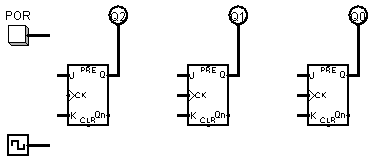
\includegraphics[width=0.7\columnwidth]{imagens/2017/contador-johnson}
\par\end{center}
\par\end{center}

}


\section{\qquestao[2]{50} Implementar um contador síncrono com a mesma sequência
da Questão \ref{sec:dg-2023-p2Contador-Sincrono-JK-1}, mas com flip-flops
tipo D. Apresentar as etapas intermediárias do projeto e o circuito
final.}

\phantom{}\hfill{}{\esptab%
\begin{tabular}{>{\centering}m{0.6cm}>{\centering}m{0.6cm}>{\centering}m{0.6cm}|>{\centering}m{0.6cm}>{\centering}m{0.6cm}>{\centering}m{0.6cm}|>{\centering}m{0.6cm}|>{\centering}m{0.6cm}|>{\centering}m{0.6cm}}
\hline 
\multicolumn{3}{c|}{Est. Pres.} & \multicolumn{3}{c|}{Est. Fut.} & \multicolumn{3}{c}{Entradas}\tabularnewline
\hline 
$Q_{2}$ & $Q_{1}$ & $Q_{0}$ & $Q_{2}$ & $Q_{1}$ & $Q_{0}$ & $D_{2}$ & $D_{1}$ & $D_{0}$\tabularnewline
\hline 
0 & 0 & 0 &  &  &  &  &  & \tabularnewline
0 & 0 & 1 &  &  &  &  &  & \tabularnewline
0 & 1 & 0 &  &  &  &  &  & \tabularnewline
0 & 1 & 1 &  &  &  &  &  & \tabularnewline
\hline 
1 & 0 & 0 &  &  &  &  &  & \tabularnewline
1 & 0 & 1 &  &  &  &  &  & \tabularnewline
1 & 1 & 0 &  &  &  &  &  & \tabularnewline
1 & 1 & 1 &  &  &  &  &  & \tabularnewline
\hline 
\end{tabular}}\hfill{}\phantom{}

\section{\questao[2]{00} Realizar a subtração por Complemento de 2 e apresentar
o resultado final em \uline{binário ``direto'' ou por Complemento
de 2 (2C)}, em\uline{ binário sinal-módulo} e em \uline{decimal}.}

\medskip{}

\begin{flushleft}
\begin{tabular*}{1\textwidth}{@{\extracolsep{\fill}}>{\centering}p{0.5\linewidth}|>{\centering}p{0.5\linewidth}}
\multicolumn{1}{>{\centering}p{0.5\linewidth}}{$\mathbf{(1\,1101)_{2}-(1\,1110)_{2}}$ \medskip{}
} & $\mathbf{(11\,0100)_{2}-(1\,1001)_{2}}$ \medskip{}
\tabularnewline
\textcolor{red}{\espv[21]} & \tabularnewline
{\small{}}%
\begin{tabular}{l|>{\centering}p{3cm}|}
\multicolumn{1}{l}{\textbf{\emph{\small{}Resultado final}}} & \multicolumn{1}{>{\centering}p{3cm}}{}\tabularnewline
\noalign{\vskip\doublerulesep}
\emph{\small{}Binário ``direto'' ou 2C:} & \tabularnewline
\cline{2-2} 
\noalign{\vskip2ex}
\emph{\small{}Binário sinal-módulo:} & \tabularnewline
\cline{2-2} 
\noalign{\vskip2ex}
\emph{\small{}Decimal:} & \tabularnewline
\cline{2-2} 
\noalign{\vskip2ex}
\end{tabular} & {\small{}}%
\begin{tabular}{l|>{\centering}p{3cm}|}
\multicolumn{1}{l}{\textbf{\emph{\small{}Resultado final}}} & \multicolumn{1}{>{\centering}p{3cm}}{}\tabularnewline
\noalign{\vskip\doublerulesep}
\emph{\small{}Binário ``direto'' ou 2C:} & \tabularnewline
\cline{2-2} 
\noalign{\vskip2ex}
\emph{\small{}Binário sinal-módulo:} & \tabularnewline
\cline{2-2} 
\noalign{\vskip2ex}
\emph{\small{}Decimal:} & \tabularnewline
\cline{2-2} 
\noalign{\vskip2ex}
\end{tabular}\tabularnewline
\end{tabular*}
\par\end{flushleft}

\texttt{\small{}}%
\begin{comment}
\texttt{\small{}Rótulo para indicar a última questão. Deixá-lo nesta
última linha e não removê-lo.}{\small\par}

\texttt{\small{}(Certamente, não deverá haver o incremento de nenhum
outro contador entre o cabeçalho da última e este rótulo \textendash{}
como, por exemplo, o de seção ou item.)}{\small\par}
\end{comment}
{\small\par}

\label{que:ultima-questao-dg-ps-2023}

\begin{comment}
an
\end{comment}

\begin{comment}
\texttt{\textbf{{*}{*}{*}{*}{*}{*}{*}{*}{*}{*}{*}{*}{*}{*}{*}{*}{*}{*}{*}{*}{*}{*}{*}{*}{*}{*}{*}{*}{*}{*}{*}{*}{*}{*}{*}{*}{*}{*}}}

\texttt{\textbf{{*}{*}{*} EXERCÍCIOS: QUESTÕES DE PROVAS {*}{*}{*}}}

\texttt{\textbf{{*}{*}{*}{*}{*}{*}{*}{*}{*}{*}{*}{*}{*}{*}{*}{*}{*}{*}{*}{*}{*}{*}{*}{*}{*}{*}{*}{*}{*}{*}{*}{*}{*}{*}{*}{*}{*}{*}}}
\end{comment}


\end{document}
